\documentclass[tikz,border=6pt]{standalone}
\usepackage{amsmath,amssymb}
\begin{document}
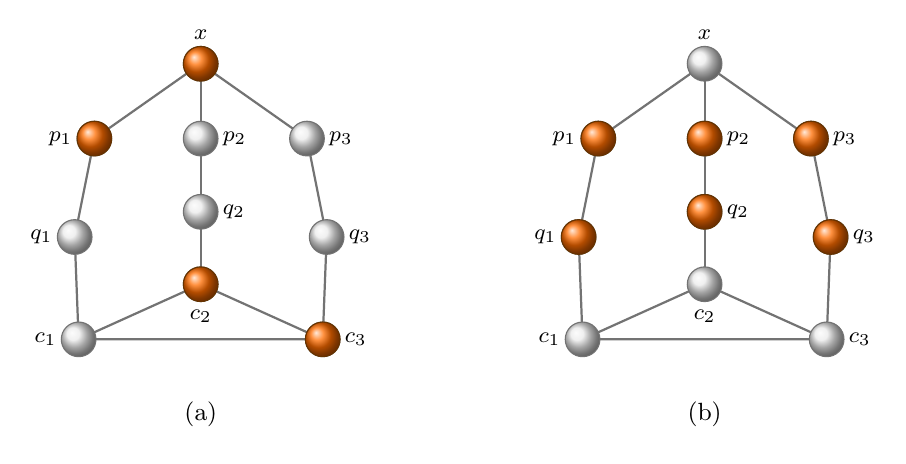
\begin{tikzpicture}[
  v/.style={circle,shading=ball,ball color=white!92!black,draw=black!55,minimum size=4.4mm,inner sep=0pt},
  d/.style={v,ball color=orange!85!red,draw=orange!40!black},
  e/.style={draw=black!55,line width=0.8pt},
  lab/.style={font=\footnotesize,inner sep=1pt}]
  \foreach \shift/\panel in {0/a,6.4/b} {
  \begin{scope}[xshift=\shift cm]
    \coordinate (x\panel) at (0,3.3);
    \coordinate (c1\panel) at (-1.55,-0.2); \coordinate (c2\panel) at (0,0.5); \coordinate (c3\panel) at (1.55,-0.2);
    \coordinate (p1\panel) at (-1.35,2.35); \coordinate (q1\panel) at (-1.6,1.1);
    \coordinate (p2\panel) at (0,2.35);     \coordinate (q2\panel) at (0,1.42);
    \coordinate (p3\panel) at (1.35,2.35);  \coordinate (q3\panel) at (1.6,1.1);
    \draw[e] (c1\panel)--(c2\panel)--(c3\panel)--(c1\panel);
    \foreach \i in {1,2,3} \draw[e] (x\panel)--(p\i\panel)--(q\i\panel)--(c\i\panel);
    \foreach \p in {x,c1,c2,c3,p1,p2,p3,q1,q2,q3} \node[v] at (\p\panel) {};
    \node[lab,above=2.6mm] at (x\panel) {$x$};
    \node[lab,left=2.4mm] at (p1\panel) {$p_1$}; \node[lab,left=2.4mm] at (q1\panel) {$q_1$};
    \node[lab,right=2.4mm] at (p2\panel) {$p_2$}; \node[lab,right=2.4mm] at (q2\panel) {$q_2$};
    \node[lab,right=2.4mm] at (p3\panel) {$p_3$}; \node[lab,right=2.4mm] at (q3\panel) {$q_3$};
    \node[lab,left=2.4mm] at (c1\panel) {$c_1$}; \node[lab,below=2.8mm] at (c2\panel) {$c_2$}; \node[lab,right=2.4mm] at (c3\panel) {$c_3$};
    \node[font=\small] at (0,-1.15) {(\panel)};
  \end{scope} }
  \foreach \p in {x,p1,c2,c3} \node[d] at (\p a) {};
  \foreach \p in {p1,p2,p3,q1,q2,q3} \node[d] at (\p b) {};
\end{tikzpicture}
\end{document}
